\documentclass[11pt,a4paper]{article}
\usepackage[margin=21mm]{geometry}
\usepackage{amsmath,amssymb,booktabs,array}
\usepackage{tikz}
\usepackage[T1]{fontenc}
\usepackage{lmodern}
\usepackage{xcolor}
\usepackage{hyperref}
\hypersetup{colorlinks=true,linkcolor=blue,urlcolor=blue}
\setlength{\parindent}{0pt}
\setlength{\parskip}{6pt}
\newcommand{\DD}{V_{\mathrm{DD}}}
\newcommand{\GND}{\mathrm{GND}}
\newcommand{\N}[1]{\mathrm{N}(#1)}
\newcommand{\Pmos}[1]{\mathrm{P}(#1)}
\newcommand{\NM}[4]{%
  \coordinate (#1t) at (#2,{#3+.5});\coordinate (#1b) at (#2,{#3-.5});
  \draw (#1t)--(#2,{#3+.28})--({#2+.12},{#3+.28})--({#2+.12},{#3-.28})--(#2,{#3-.28})--(#1b);
  \draw ({#2-.14},{#3-.2})--({#2-.14},{#3+.2});
  \draw ({#2-.55},#3)--({#2-.14},#3);
  \node[anchor=east] at ({#2-.62},#3) {$#4$};}
\newcommand{\PM}[4]{%
  \coordinate (#1t) at (#2,{#3+.5});\coordinate (#1b) at (#2,{#3-.5});
  \draw (#1t)--(#2,{#3+.28})--({#2+.12},{#3+.28})--({#2+.12},{#3-.28})--(#2,{#3-.28})--(#1b);
  \draw ({#2-.14},{#3-.2})--({#2-.14},{#3+.2});
  \draw ({#2-.55},#3)--({#2-.35},#3);
  \draw ({#2-.295},#3) circle[radius=.055];
  \draw ({#2-.24},#3)--({#2-.14},#3);
  \node[anchor=east] at ({#2-.62},#3) {$#4$};}
\newcommand{\groundat}[2]{\draw (#1,#2)--(#1,{#2-.13});
  \draw ({#1-.28},{#2-.13})--({#1+.28},{#2-.13});
  \draw ({#1-.18},{#2-.22})--({#1+.18},{#2-.22});
  \draw ({#1-.08},{#2-.31})--({#1+.08},{#2-.31});}
\newcommand{\AOIcircuit}[5]{%
\begin{tikzpicture}[line width=.8pt,x=.9cm,y=.9cm]
  \PM{P1}{.8}{6.1}{#1}\PM{P2}{3.8}{6.55}{#2}\PM{P3}{3.8}{5.45}{#3}
  \PM{P4}{.8}{3.95}{#4}\PM{P5}{3.8}{3.95}{#5}
  \draw (.8,7.2)--(3.8,7.2);\draw (2.3,7.2)--(2.3,7.5) node[above] {$\DD$};
  \draw (P1t)--(.8,7.2);\draw (P2t)--(3.8,7.2);\draw (P2b)--(P3t);
  \draw (P1b)--(.8,4.8)--(3.8,4.8)--(P3b);
  \draw (P4t)--(.8,4.8);\draw (P5t)--(3.8,4.8);
  \draw (P4b)--(.8,3.2)--(3.8,3.2)--(P5b);
  \draw (3.8,3.2)--(5.1,3.2) node[right] {$f$};
  \fill (3.8,3.2) circle[radius=.05];
  \NM{N1}{.8}{2.4}{#1}\NM{N2}{0}{1}{#2}\NM{N3}{1.7}{1}{#3}
  \NM{N4}{3.8}{2.4}{#4}\NM{N5}{3.8}{1}{#5}
  \draw (N1t)--(.8,3.2);\draw (N4t)--(3.8,3.2);\draw (N4b)--(N5t);
  \draw (N1b)--(.8,1.7);\draw (0,1.7)--(1.7,1.7);
  \draw (N2t)--(0,1.7);\draw (N3t)--(1.7,1.7);
  \draw (N2b)--(0,.3)--(3.8,.3)--(N5b);\draw (N3b)--(1.7,.3);
  \groundat{2.3}{.3}
  \node[anchor=west,font=\small,text=gray] at (5.1,5.5) {PUN};
  \node[anchor=west,font=\small,text=gray] at (5.1,1.7) {PDN};
\end{tikzpicture}}

\begin{document}

\begin{center}{\Large\bfseries 2013 Homework 3}\par Fixed-size transmission-gate MUX and inverter short-circuit power\end{center}
The original printed prompt is preserved at \texttt{../assignments/homework3.pdf}.
Both supplied DOCX versions of the 100501015 answer were read, including their
embedded plots. The original 10 fF load and fixed TG dimensions are followed here.

\section*{1. Baseline 8:1 transmission-gate multiplexer}
Set $S=s_0+2s_1+4s_2$ and require $z=a_S$. Every TG uses the specified
$W_n=10\,\mu$m, $W_p=20\,\mu$m and $L=0.18\,\mu$m. It contains parallel
NMOS/PMOS channels, enabled by complementary gates. Generate each $\bar s_i$
once with a shared CMOS inverter. All PMOS bodies connect to VDD and NMOS
bodies to ground; the load is exactly 10 fF.

The baseline provides eight separate three-TG paths, each decoding one select
word. Its 24 TGs plus three select inverters require $48+6=54$ MOSFETs.
The selected path crosses three TGs; inactive paths add capacitance at their
shared output. Use the same 10 fF output load and 20 ps data slew for both designs.

\begin{center}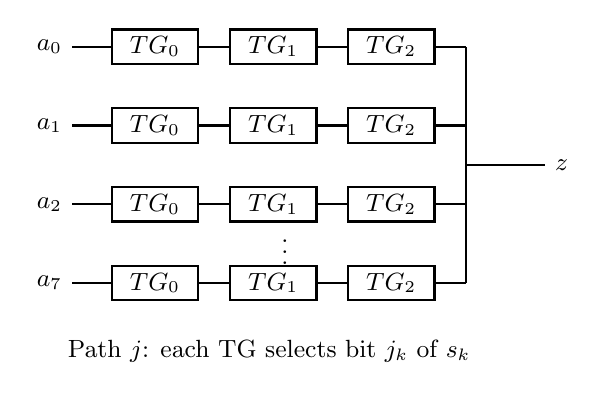
\begin{tikzpicture}[line width=.8pt,font=\small]
\foreach \j/\y in {0/3,1/2,2/1,7/0}{
 \node[left] at (0,\y) {$a_\j$};\draw (0,\y)--(.5,\y);
 \foreach \k in {0,1,2}{\draw ({.5+1.5*\k},{\y-.22}) rectangle ({1.6+1.5*\k},{\y+.22});
 \node at ({1.05+1.5*\k},\y) {$TG_\k$};\draw ({1.6+1.5*\k},\y)--({2+1.5*\k},\y);}
}
\draw (5,0)--(5,3);\draw (5,1.5)--(6,1.5) node[right] {$z$};
\node at (2.7,.5) {$\vdots$};\node[below] at (2.5,-.6) {Path $j$: each TG selects bit $j_k$ of $s_k$};
\end{tikzpicture}\end{center}
The diagram abbreviates the middle four paths. Their complete connections,
dimensions and control polarities are in the standalone \texttt{mux.sp}.

\section*{Improved topology with unchanged TG sizes}
Replace the separate paths by a binary 2:1 tree: four first-stage muxes select
adjacent data pairs with $s_0$; two second-stage muxes use $s_1$; one final mux
uses $s_2$. Each 2:1 mux uses two TGs. Thus the improved network has 14 TGs and
three shared inverters, or $28+6=34$ MOSFETs. The depth remains three TGs,
but only two final TG terminals load the output instead of eight.
\begin{center}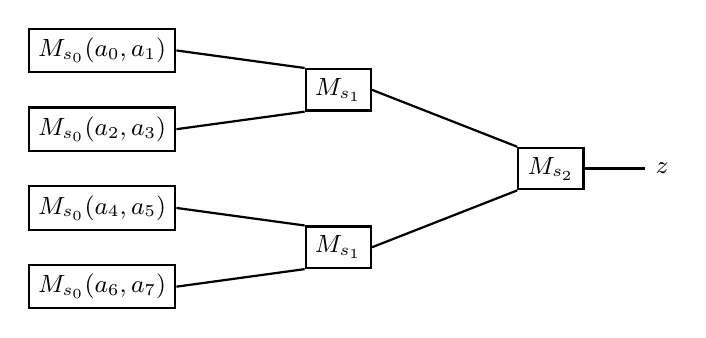
\begin{tikzpicture}[line width=.8pt,font=\small]
\foreach \j/\y in {0/3,1/2,2/1,3/0}{\pgfmathtruncatemacro{\lo}{2*\j}\pgfmathtruncatemacro{\hi}{2*\j+1}\node[draw,minimum width=18mm] (m\j) at (0,\y) {$M_{s_0}(a_{\lo},a_{\hi})$};}
\node[draw] (n0) at (3,2.5) {$M_{s_1}$};\node[draw] (n1) at (3,.5) {$M_{s_1}$};
\node[draw] (o) at (5.7,1.5) {$M_{s_2}$};
\draw (m0.east)--(n0.north west);\draw (m1.east)--(n0.south west);
\draw (m2.east)--(n1.north west);\draw (m3.east)--(n1.south west);
\draw (n0.east)--(o.north west);\draw (n1.east)--(o.south west);\draw (o.east)--(6.9,1.5) node[right] {$z$};
\end{tikzpicture}\end{center}
Each $M_s$ passes its lower-index data when $s=0$ and its higher-index data
when $s=1$. No TG transistor is resized to obtain the improvement.

\newpage\section*{Actual HSPICE delay comparison}
Conditions: CIC018 TT, 1.8 V, $25^\circ$C, 10 fF output load, 20 ps input
0--100\% slew, 1 ps maximum timestep. Each of eight settled select words is
tested with the selected data rising and falling, all other data held low.
Both designs run in the same sweep with independent loads. Propagation delay
is the last output 0.9 V crossing minus the input 0.9 V crossing.
\begin{center}\begin{tabular}{crrrr}\toprule
Select&Baseline LH&Baseline HL&Tree LH&Tree HL\\&ps&ps&ps&ps\\\midrule
0&212.257&203.307&66.352&76.191\\
1&213.822&201.262&68.550&73.761\\
2&215.152&201.274&68.285&74.978\\
3&216.681&199.180&70.416&72.510\\
4&216.298&200.784&67.063&75.130\\
5&217.825&198.714&69.242&72.682\\
6&219.019&198.684&68.982&73.898\\
7&220.507&196.567&71.084&71.416\\
\bottomrule\end{tabular}\end{center}
\[
 \boxed{t_{\max,baseline}=220.507\ \mathrm{ps},\quad
 t_{\max,tree}=76.191\ \mathrm{ps}.}
\]
The measured worst-case reduction is 65.447\%. Every one of the 16
paired transition tests shows an improvement. Before/after levels pass low
$\le0.2$ V and high $\ge1.6$ V. These maxima apply to the declared data-edge
tests; select-switching hazards and PVT extremes are not claimed to be covered.
An independent Boolean tree evaluation checks all $8\times256=2048$ legal
select/data combinations. Its truth evidence is not mislabeled as 2048
physical HSPICE experiments.

\textbf{Reference comparison.} The supplied answer correctly proposes a
shared binary tree. However, its baseline lists a 1 fF load rather than the
printed 10 fF; the improved code omits the load, and its data slew changes
from 200 ps to 100 ps. Those experiments cannot establish a matched-condition
speedup. We retain the tree idea, share select complements, use the same
required load and stimuli, and measure both directions for every select word.
Reported reference delays 241.765/78.465 ps are not reused as our measurements.

\section*{Reproduce and evidence}
Run \texttt{python reproduce.py} with \texttt{--model D:/cic018.l} and
\texttt{--work PATH}. The optional \texttt{--hspice} flag selects another
installation. \texttt{--prepare-only} regenerates the 2048-case logic table
and decks without claiming a simulator run. The reusable circuit is
\texttt{mux.sp}; both testbenches use the local process library.
\texttt{results/summary.json}, \texttt{mux\_delays.csv},
\texttt{inverter\_power.csv} and \texttt{logic\_2048.csv} preserve the checks.
Raw simulator and license logs remain outside the repository. No process
model or layout artifacts are published.

\newpage\section*{2. Short-circuit power versus load capacitance}
Choose inverter $W_p=20\,\mu$m, $W_n=10\,\mu$m, $L=0.18\,\mu$m; its
sizes are not specified by this part of the prompt. Use 1.8 V, TT, $25^\circ$C,
the required 3 ns rising and falling input ramps, and a declared 20 ns period.
The corrected single capacitor is parameterized at the inverter's actual
output for $C_L=0.1,0.3,0.5,0.7,1.0$ pF.

During an input transition, NMOS and PMOS can both conduct. Separately from
capacitive charging, estimate their common through-channel current using
HSPICE's intrinsic channel-current outputs, LX4:
\[
 I_{sc}(t)=\max\{0,\min[I_{p,ch}(t),I_{n,ch}(t)]\},\qquad
 P_{sc}=\frac{V_{DD}}{T}\int_{t_0}^{t_0+T}I_{sc}(t)\,dt.
\]
LX4 is positive for the normally biased PMOS and NMOS here; the outer clamp
removes reverse-bias/overshoot values. This is an explicitly declared
channel-overlap estimator, not total transistor dissipation, terminal
displacement current, an edge-window average, or peak power. Average a complete
settled cycle from 23 to 43 ns. Supply power is measured independently as
$\langle-V_{DD}I(VDD)\rangle$. External-load switching power is $C_LV_{DD}^2/T$.

\begin{center}\begin{tabular}{rrrr}\toprule
$C_L$ (pF)&$P_{sc}$ ($\mu$W)&Supply power ($\mu$W)&$C_LV_{DD}^2/T$ ($\mu$W)\\\midrule
0.1&113.373082&138.184419&16.200000\\
0.3&100.912372&158.139075&48.600000\\
0.5&91.925520&181.573889&81.000000\\
0.7&84.947117&207.021195&113.400000\\
1.0&76.828513&247.545707&162.000000\\
\bottomrule\end{tabular}\end{center}
\begin{center}\begin{tikzpicture}[x=7cm,y=.034cm]
\draw[->] (0,0)--(1.12,0) node[right] {$C_L$ (pF)};
\draw[->] (0,0)--(0,150) node[above] {$P_{sc}$ ($\mu$W)};
\foreach \x in {.1,.3,.5,.7,1}{\draw (\x,0)--(\x,-2) node[below] {$\x$};}
\foreach \y in {0,40,80,120}{\draw (0,\y)--(-.015,\y) node[left] {$\y$};\draw[gray!25] (0,\y)--(1.05,\y);}
\draw[blue,thick] plot coordinates {(0.1,113.373082) (0.3,100.912372) (0.5,91.925520) (0.7,84.947117) (1,76.828513)};
\end{tikzpicture}\end{center}
The measured overlap power decreases as the load grows for this fixed input
slew and sizing. During the input's overlap interval, a larger load keeps the
output closer to its previous rail, reducing the drain-source voltage of one
of the conducting devices and limiting direct through current. Meanwhile,
external-load switching power increases linearly with $C_L$; total supply
power must therefore be distinguished from $P_{sc}$. A universal monotonic
law for arbitrary slew, size and activity is not claimed.

\textbf{Reference correction.} The supplied inverter uses node \texttt{out},
but its altered capacitors are connected to \texttt{vout}; the original
0.1 pF capacitor remains unchanged. It also averages \texttt{P(MOS)} over
changing edge windows. Thus its load sweep and listed powers do not reproduce
the required cycle-average short-circuit curve. The corrected experiment
changes one actual load and records intrinsic-current overlap and supply
power separately. All five sampled high/low output levels are valid.


\end{document}
